\documentclass[12pt,letterpaper]{article}
\usepackage{amsmath}
\usepackage{amsfonts}
\usepackage{appendix}
\usepackage[figurewithin=section,tablewithin=section]{caption}
\usepackage[usenames,dvipsnames]{color}
\usepackage{graphicx}
%\usepackage{epsfig}
%\usepackage{epstopdf}
%\usepackage[outdir=./]{epstopdf}
\usepackage{longtable}
\usepackage{rotating}
\usepackage{booktabs}
\usepackage[bibencoding=utf8, citestyle=authoryear,bibstyle=authoryear,maxbibnames=99]{biblatex}
%\addbibresource{~/Projects/MyBibtex.bib}

\bibliography{/home/jsibert/Projects/MyBibtex.bib,/home/jsibert/MendeleyBibTex/library.bib}

\usepackage[pdftex,bookmarks=false]{hyperref}
\hypersetup{pdfauthor={John Sibert}
            pdfsubject={variable transmission and mortality rate estimates}
            pdftitle={Simple SIR Statistical Model}
            pdfkeywords={Covid-19, SIR Model, random effects, TMB}
            }%

\newcommand\doublespacing{\baselineskip=1.6\normalbaselineskip}
\newcommand\singlespacing{\baselineskip=1.0\normalbaselineskip}
\newcommand\help[1]{\color{Magenta}{\it #1 }\normalcolor}
\newcommand\EG{e.g.\ }
\newcommand\perda{$\rm{da}^{-1}$}
\newcommand\SSm{{\tt simpleSIR4}}
\newcommand\slI{$\sigma_{\ln I}$\ }
\newcommand\slD{$\sigma_{\ln D}$}
\newcommand\slB{$\sigma_{\ln \beta}$}
\newcommand\slM{$\sigma_{\ln \mu}$}

%\renewcommand{\appendixtocname}{Supplementary Material}

\title{Trends in transmission and mortality rates of the Covid-19
pandemic estimated from publicly available data}

\author{
John Sibert\thanks{sibert@hawaii.edu; johnrsibert@gmail.com}\\
Joint Institute of Marine and Atmospheric Research\\
University of Hawai`i at M\={a}noa\\
Honolulu, HI  96822 U.S.A.\\[0.125in]
\date{\today}
}

\pagestyle{headings}
\markright{John Sibert \hfil Covid-19 Transmission \& Mortality \hfil \today}

\begin{document}

\maketitle

\doublespacing

\begin{abstract}
A simple compartment model of Covid-19 infections and deaths is
applied to publicly available data to estimate trends and transmission
and mortality rates using random effects. Model estimates of
infections and deaths match observations closely. Trends in
estimated transmission rate vary substantially between geographic
areas. Transmission rates were suppressed below 0.007\perda\ by the
end of May in some areas, but often rebounded when social constraints
were relaxed.
Mortality rates of individuals infected with Covid-19 fell to less than
0.001\perda\ in most areas by the end of July.
These results show that publicly available data, often collected and
compiled with different protocols, can be used to quantitatively
estimate trends in transmission and mortality rate.
\end{abstract}

\section*{Introduction}

The sudden advent of the Covid-19 pandemic provoked many political
jurisdictions to advise people to ``shelter in place'' and to practice
``social distancing''. If this advice has been effective, it should be
possible to detect the effects of the advice by comparing changes in
transmission rates over time and between areas. 
SIR models are often applied to the spread of epidemics and have
certainly been applied to the current Covid-19 pandemic
(e.g. \cite{Chen2020,Roques2020}).
These models divide the affected the effected population into three
compartments: susceptible (S), Infected (I) and Recovered (R).
SIR models are
usually expressed as coupled ordinary differential equations,
\begin{eqnarray}
\label{eqn:SIR}
\frac{dS}{dt} &=& -\beta\frac{IS}{N} - \mu S\\
\frac{dI}{dt} &=& \hphantom{-}\beta\frac{IS}{N} - \mu I -\gamma I\\
\frac{dR}{dt} &=&  -\mu R +\gamma I\\
N &=& S + I + R
\end{eqnarray}
where $N$ is the population size, $\beta$ is the instantaneous
rate ($[t^{-1}]$), $\mu$ is the instantaneous mortality rate
($[t^{-1}]$),
and $\gamma$ is the instantaneous recovery rate ($[t^{-1}]$).  

%https://en.wikipedia.org/wiki/Compartmental_models_in_epidemiology

As the pandemic began to unfold, scientific institutes and governments
at different levels began to make data publicly available on the
World Wide Web.
Unfortunately, data collection protocols may vary between
institution over time. Additionally, few data sets include data for each of
the compartments in a SIR model. 
The New York Times' ``historical'' 
data set\footnote{\label{ff:nyt}\url{https://github.com/nytimes/covid-19-data/}}
is an easily accessible source of data and is updated daily. These data
comprise daily totals of ``cases'' and ``deaths'' for each county
in the United States. I assume that the data included as ``cases'' are
a reasonable approximations of the Infected compartment ($I$) in a SIR
model. There are simply no credible data of comparable scope on
either the Susceptible or the Recovered compartments.

\section*{Model Structure}
I make some simplifying assumptions in the face of incomplete data: 
(1) The entire population is susceptible so that $S/N = 1$. 
(2) Over the short term, the size of the
Susceptible compartment does not change, 
$\frac{dS}{dt} = 0 = \frac{dN}{dt}$,
eliminating the Susceptible compartment.
(3) People who recover from a Covid-19 infection return to the Susceptible
compartment, eliminating the Recovered compartment. 
With these assumptions, and with the addition of a ``deaths''
compartment, the simplified SIR model is
\begin{eqnarray}
\label{eqn:sSIRI}
\frac{dI}{dt} &=&  \beta I - \mu I -\gamma I\\
\label{eqn:sSIRD}
\frac{dD}{dt} &=& \mu I
\end{eqnarray}
Most importantly this model
has state variables that might be matched to available observations.

The available data contain measurement errors of various types.
Definitions and methods of detecting and reporting the numbers of
infected persons and numbers of deaths attributable to Covid-19 have
changed since January of 2020, are continuing to evolve, and can be
expected to change in the future.
Reporting protocols also vary between political jurisdictions (or
``geographies'' in the parlance of the New York Times).
Finally, there is additional variability in the biosocial
processes that mediate disease transmission.

State-space models separate variability in the biosocial
processes in the system (transition model)
from errors in observing features of interest
in the system (observation model).
(See \cite{Harvey1990}).

The general form of a state-space process or transition model is
\begin{equation}
\alpha_t=T(\alpha_{t-1}) + \Theta_t
\end{equation}
where $\alpha_t$ is the state at time $t$ and 
the function $T$ embodies the dynamics mediating the
development of the state at time $t$ from the state at the previous
time with random process error, $\Theta_t$.

The transition model for the simplified SIR model is constructed from
the explicit finite difference
approximations of equations~(\ref{eqn:sSIRI}) and~(\ref{eqn:sSIRD}) 
with associated log-normal
random errors.
\begin{eqnarray}
\label{eqn:sSIRfdI}
I_t &=& I_{t-\Delta t}\big(1+\Delta t(\beta_{t-\Delta t} - \mu_{t-\Delta t}
- \gamma_{t-\Delta t})\big)e^{\eta_t}\\
\label{eqn:sSIRfdD}
D_t &=& \big(D_{t-\Delta t} + \Delta t \mu_{t-\Delta t}I_{t-\Delta
t}\big)e^{\eta_t}
\end{eqnarray}
where $\eta$ is a normal random deviate, $\eta\sim
N(0,\sigma_\eta)$, representing temporal variability in the biosocial
factors that mediate the spread of the pandemic. 
I have no particular justification, beyond the parsimony principle,
for the assumption that the variance, $\sigma_\eta$, of the processes
for $I$ and $D$, should be the same.

The rate constants in the SIR model differential equations (in this
case $\beta$, $\mu$ and $\gamma$) are often assumed to be invariant.
This biological assumption clearly conflicts with the social
assumptions
that behavioral modification can reduce transmission rates and
that medical advances can reduce both transmission and mortality
rates.
One approach to modeling time-dependent rates of transmission and
mortality, $\beta$ and $\mu$, is to treat them as random effects
(\cite{Skaug2006}). Random effects are appropriate if repeating a time
series of observations would not yield the same outcome as the initial
observations. Random effects are also appropriate when observing
the same process in two different areas. I model the  $\beta$ and
$\mu$ time series as log-normal random walks. I assume that
\begin{eqnarray}
\log\beta_t &=& \log\beta_{t-\Delta t}+\varepsilon;\quad \varepsilon\sim 
N(0,\sigma_\beta)\\
\log\mu_t &=& \log\mu_{t-\Delta t}+\varrho;\quad \varrho\sim
N(0,\sigma_\mu)
\end{eqnarray}
A similar approach has been used by fisheries scientists to represent
ill-determined parameters in fisheries stock assessment models, such
as time-dependent fishing induced mortality
(\cite{Nielsen2014b,Sibert2017}).

The recovery rate, $\gamma_{t-\Delta t}$, in equation
(\ref{eqn:sSIRfdI}) is computed algebraically as
\begin{equation}
\gamma_{t-\Delta t} = \beta_{t-\Delta t} - \mu_{t-\Delta t} +
(1-\frac{I_t}{I_{t-\Delta t}})
\end{equation}

The general form of the state-space observation model is
\begin{equation}
x_t = O(\alpha_t) + \Omega_t
\end{equation}
where the function $O$ describes the measurement process with
error $\Omega$ in observing the state $\alpha$.

I applied separate observation error models for cases and
deaths. The observation model for cases is a simple log-normal error
\begin{equation}
\label{eqn:logNlike}
\log\varphi_t = \bigg(\log\frac{1}{\sqrt{2\pi\sigma^2_I}} -\Bigl(\frac{\log
I_t-\log\widehat{I}_t}{\sigma_I}\Bigr)^2\bigg)\\
\end{equation}
where $I$ is the observed number of cases and $\widehat{I}$ is the
number of cases predicted by equation~\ref{eqn:sSIRfdI}.


Not all those afflicted by Covid-19 have died; there are far fewer
deaths than infections. In addition,
the observed time series for both $I$ and $D$ begins at the first recorded
case, i.e. at time $t=0, I_t \ge 1$. The first recorded death occurs
several days or weeks after the first recorded case.
Therefore the deaths time-series inevitably contains a
substantial number of initial recorded zeros. 
The observation model for deaths accommodates observed zeroes by
assuming to be ``zero-inflated'' log normal likelihood given by
\begin{equation}
\label{eqn:ZIlogNlike}
  \log \varepsilon_t = \left\{
    \begin{array}{r@{\;:\quad}l}
       D_t > 0 &
(1-p_0)\cdot\bigg(\log\frac{1}{\sqrt{2\pi\sigma^2_D}}
          -\Bigl(\frac{\log D_t-\log\widehat{D}_t}{\sigma_D}\Bigr)^2\bigg)\\
       D_t = 0 & p_0 \cdot\log \frac{1}{\sqrt{2\pi\sigma^2_D}}\\
    \end{array}
  \right.
\end{equation}
where $D$ is the observed number of deaths,
$\widehat{D}$ is the number of deaths predicted by
equation~\ref{eqn:sSIRfdD}, 
and $p_0$ is the proportion of observed deaths equal to zero.

\begin{table}
\caption{List of model variables for the simple SIR model, \SSm.
There are two state variables computed from the of estimated
parameters and random effects.
There are two random effects and five estimated variance parameters.
All models variables are represented in the TMB C++ module as their
natural logarithms.
}
\label{tab:allvars1}
\begin{center}
\begin{tabular}{ll}
\hline
Variable & Definition\\
\hline
\hline
       & {\it State variables:}\\
$I$      & Number of infected individuals\\
$D$      & Number of deaths\\
       & {\it Random effects:}\\
$\beta_t$ & Transmission rate; log-normal random walk\\
$\mu_t$   & Mortality rate; log-normal random walk\\
       & {\it Estimated parameters:}\\
$\sigma_I$ & Infectious compartment estimation standard deviation\\
$\sigma_D$ & Deaths compartment estimation standard deviation\\
$\sigma_\eta$ & Standard deviation of transmission and deaths process errors\\
$\sigma_\beta$ & Standard deviation of transmission rate random walk\\
$\sigma_\mu$ & Standard deviation of mortality rate random walk\\
\hline
\end{tabular}
\end{center}
\end{table}

Model parameters are estimated by
maximizing the joint likelihood of the process errors, observation
errors, and random effects.
\begin{equation}
\label{eqn:likelihood}
L(\theta,\alpha,x)=
\prod^m_{t=1}\big[\phi\big(\alpha_t-T(\alpha_{t-1}), \Theta\big)\big]\cdot
\prod^m_{t=0}\big[\phi\big(x_t-O(\alpha_t), \Omega\big)\big]
\end{equation}
where $m$ is the number of days elapsed since the first recorded case,
$x_t$ is the vector of daily observations of cases and deaths,
$\alpha_t$ is the vector of the daily calculations of the state
variables and random effects,
and $\theta$ 
is a vector of model parameters (Table~\ref{tab:allvars1}).
The R package TMB (\cite{TMB0000}) was used to 
estimate the parameters of the model. 
The R and supporting C++ files are available on 
github.\footnote{\SSm~at \url{https://github.com/johnrsibert/SIR-Models}}

%\clearpage
\section*{Results}

\begin{figure}[h!]
\begin{center}
\includegraphics[width=1.00\textwidth]{../Graphics/constrainID/counties_per_capita.pdf}
\end{center}
\caption{\label{fig:percap}
Trends in number of cases per 1000 people in the 30 most populous US
counties.
The vertical gray bar mark the March 19, 2020 California shelter in place order.
See Table~\ref{tab:namekey} for key to county abbreviations.
}
\end{figure}

%All data are derived from the New York times github 
%site\footnote{See note \ref{ff:nyt}.}.
% {\url{https://github.com/nytimes/covid-19-data/}}. 

Six months after the pandemic began spreading in the United States, it
was obvious that some areas were more successful than other
in controlling the spread of the Covid-19 virus.
Trends in the per-capita number of cases in the thirty most populous 
counties in the
United States are shown in Figure~\ref{fig:percap}.
These trajectories fall into two more or less distinct groups: those
that are concave downward, \EG Nassau Co. NY (NaNY), indicating
successful control, and those that are
concave upward, \EG Miami-Dade Co. FL (MDFL), indicateing less
successful control.


\begin{figure}
{\scriptsize
\begin{center}
\includegraphics[width=0.80\textwidth]{../Graphics/constrainID/NassauNY_prevalence.png}
 
\vspace{0.25truein}

\includegraphics[width=0.80\textwidth]{../Graphics/constrainID/Miami-DadeFL_prevalence.png}
\end{center}
}
\caption{\label{fig:prev}
Prevalence trajectories for two US counties.
Blue bars indicate daily increases increases in cases and deaths;
dark blue lines enclosing the bars indicate 11 day moving averages of
daily increases (labeled ``11da'');
pale blue lines indicate cumulative numbers (labeled $\Sigma C$ and
$\Sigma D$); 
vertical gray bar marks the March 19, 2020 California shelter in place order.
}
\end{figure}

Prevalence histories for counties representative of concave
downward and concave upward trajectories are shown in
Figure~\ref{fig:prev}. The 11-day moving averages of the daily
increases in cases and deaths is a good indicator of the
relative success in controlling the outbreak.
The cumulative trends in number of cases is equivalent to 
the per capita trends in Figure~\ref{fig:percap}.
All histories show extreme day to day variability.
Variability is most notable in the deaths
time series, particularly for smaller counties.

The \SSm\  model estimates two random effects and five parameters.
In principle, all random effects and parameters are estimated
simultaneously.
Initial experiments with the model showed that several different
numerical algorithms used to find the minimum of the log likelihood
function were unable to easily reach a solution. Minima were reached
for some counties, but most attempts terminated prematurely. 
Inspection of the diagnostic plots for the model showed that predicted
values of cases and deaths matched observed values almost exactly
with unrealistically low estimates of \slI and \slD.
The extreme variability in the data is reflected in the extreme
variability of the estimated trends in transmission and mortality
rates estimated by the unconstrained 5 parameter model.
See Appendix figures~\ref{fig:estsNaNYu} and~\ref{fig:estsMDFLu}
for details.

The \SSm\ model is easily configured with selected parameters fixed at
constant values. 
All subsequent analysis focused on models with 
\slI~$ = 0.223$ and \slD~$= 0.00953$. 
These standard deviations are equivalent to measurement errors of
approximately 25\% in reporting cases and 10\% in reporting deaths.
The algorithm converges to a solution in all cases, and converges
rapidly using gradient methods.

\begin{figure}
\begin{center}
\includegraphics[width=1.00\textwidth]{../Graphics/constrainID/NassauNY_TMB_estimates_a.pdf}
\end{center}
\caption{\label{fig:estsNaNYc}
Diagnostic plots of model estimates for Nasssau County, NY, 
with constraints of the observation model variance, 
\slI~$ = 0.223$ and \slD~$= 0.00953$. 
See page~\pageref{pp:diagexpl} for explanation of figure.
}
\end{figure}

\begin{figure}
\begin{center}
\includegraphics[width=1.00\textwidth]{../Graphics/constrainID/Miami-DadeFL_TMB_estimates.pdf}
\end{center}
\caption{\label{fig:estsMDFLc}
Diagnostic plots of model estimates for Miami-Dade County,FL,
with constraints of the observation model variance, 
\slI~$ = 0.223$ and \slD~$= 0.00953$. 
See page~\pageref{pp:diagexpl} for explanation of figure.
}
\end{figure}

\label{pp:diagexpl} 
Diagnostic information for the model estimates is plotted
%(figures~\ref{fig:estsNaNYc} and~ \ref{fig:estsMDFLc})
on logarithmic scales both to illustrate the
lognormal likelihood functions used in the observation model,
equations (\ref{eqn:logNlike}) and (\ref{eqn:ZIlogNlike}) and to
illustrate trends in estimated transmission and mortality rates close
to zero.
The blue `+' symbols represent the observed cases ($I$) and deaths ($D$).
The red lines overlaying the symbols are model predictions ($\widehat{I}$)
and ($\widehat{D}$) of cases and deaths. 
%$\sigma_I$ and $\sigma_D$ are the estimated standard deviations of
%logarithms of cases and deaths in the observation model.
The shaded areas bounded by red outlines are 
$\pm 2$ estimated standard deviations, \slI\ and \slD\ in the
observation model, around the estimated trends.
The solid blue lines in the transmission rate $\ln \beta$ and
mortality rate $\ln \mu$ diagnostic plots are the estimated
transmission and death rate random effects.
The shaded areas bounded by blue outlines are
estimated random effects $\pm 2$ estimated standard errors of the
random effect.
%, \slB\ and \slM, of the generating random walks in the transition model.
%These areas should not be considered as indicators of the precision
%of the estimated random effects.
The red lines labeled $\tilde{\beta}$ and $\tilde{\mu}$ are the
medians of the estimated random effects over the time period.

Diagnostic plots for the constrained model are shown in
figures~\ref{fig:estsNaNYc} and~ \ref{fig:estsMDFLc}
for convex downward and convex upward trajectories
respectively.
Estimated cases and deaths agree well with observation throughout the
time series because of constraints on the observation model errors.
Distinct trends in transmission rate estimates are plainly evident for
the two prevalence patterns. A small, but distict, 
transitory upward ``bump'' in July is
evident for the convex downward example, Miami-Dade Co. FL.
Estimated mortality rates trend generally downward  for both patterns.

\begin{figure}[h!]
\begin{center}
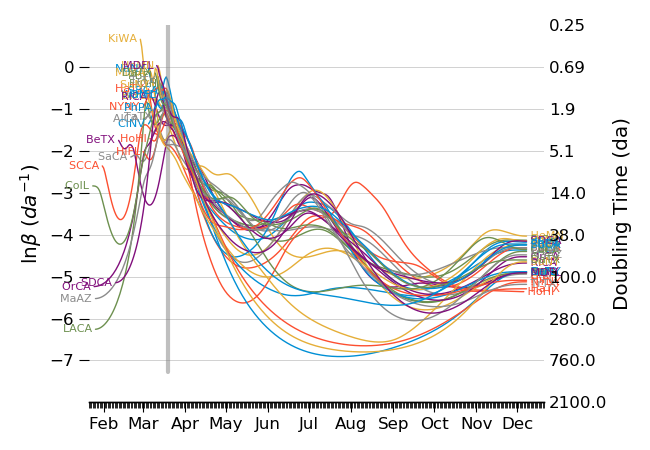
\includegraphics[width=1.00\textwidth]{../Graphics/constrainID/logbeta_summary_g.pdf}\\
\end{center}
\caption{\label{fig:xrates}
Estimated natural logarithms of the transmission rate for thirty two US
counties using the constrained \SSm\ model.
Equivalent doubling times ($t_2 = \frac{\ln 2}{\exp(\ln \beta)}$)
are shown on the right-hand ordinate.
See Table~\ref{tab:namekey} for key to county abbreviations.
}
\end{figure}

Figure~\ref{fig:xrates} compares estimated transmission rate among
counties.
Transmission rates increased rapidly immediately after the first
recorded case, and by early March the instantaneous transmission rate was greater
than 1\perda\ ($\ln \beta \approx 0$),
equivalent to a doubling time of less than one day.
Beginning in April, transmission rates fell substantially, and doubling times
increased to longer than 20 days in some counties by late May.
Counties with estimated transmission rates less than 0.007\perda\ 
(or $\ln \beta \le 5$) at the end of May
correspond roughly to those counties with concave downward prevalence
trajectories.
Figure~\ref{fig:xrates2} is a simplified presentation of estimated
transmission rate between counties that compare counties with sustainable
suppression of transmission (Cook Co, IL, Nassau Co, NY) with two counties that
have suffered a resurgence of cases (Honolulu Co, HI and Miami-Dade Co
FL). The Honolulu example indicates that simply suppressing the
transmission rate to a point where the doubling time is greater than
100 days does not ensure a sustainable outcome. The regions encolsed
by $\pm 2$ standard errors show that estimated transmission rates these four counties
were similar in April and May, but diverged significantly in June to
become distinct in August.

\begin{figure}[h!]
\begin{center}
\includegraphics[height=0.40\textheight]{../Graphics/constrainID/logbeta_summary.pdf}\\
%\includegraphics[width=1.00\textwidth]{../Graphics/constrainID/logbeta_summary.pdf}\\
\end{center}
\caption{\label{fig:xrates2}
Estimated natural logarithms of the transmission rate for four US
counties using the constrained \SSm\ model.
The shaded areas indicate the estimated random effect $\pm 2$
estimated standard errors.
Equivalent doubling times ($t_2 = \frac{\ln 2}{\exp(\ln \beta)}$)
are shown on the right-hand ordinate.
See Table~\ref{tab:namekey} for key to county abbreviations.
}
\end{figure}

Figure~\ref{fig:drates} compares estimated mortality rate among
counties. Initial mortality rates were quite variable during the first
months of the pandemic and but rose quickly to around 
0.01\perda\ ($\ln \mu \approx 4.6$) in April. Subsequently the
estimated mortality rates decreased similarly for all counties and appear to
have leveled off in August to lows near
0.0003\perda\ ($\ln \mu \approx -8$) in August.

\begin{figure}
\begin{center}
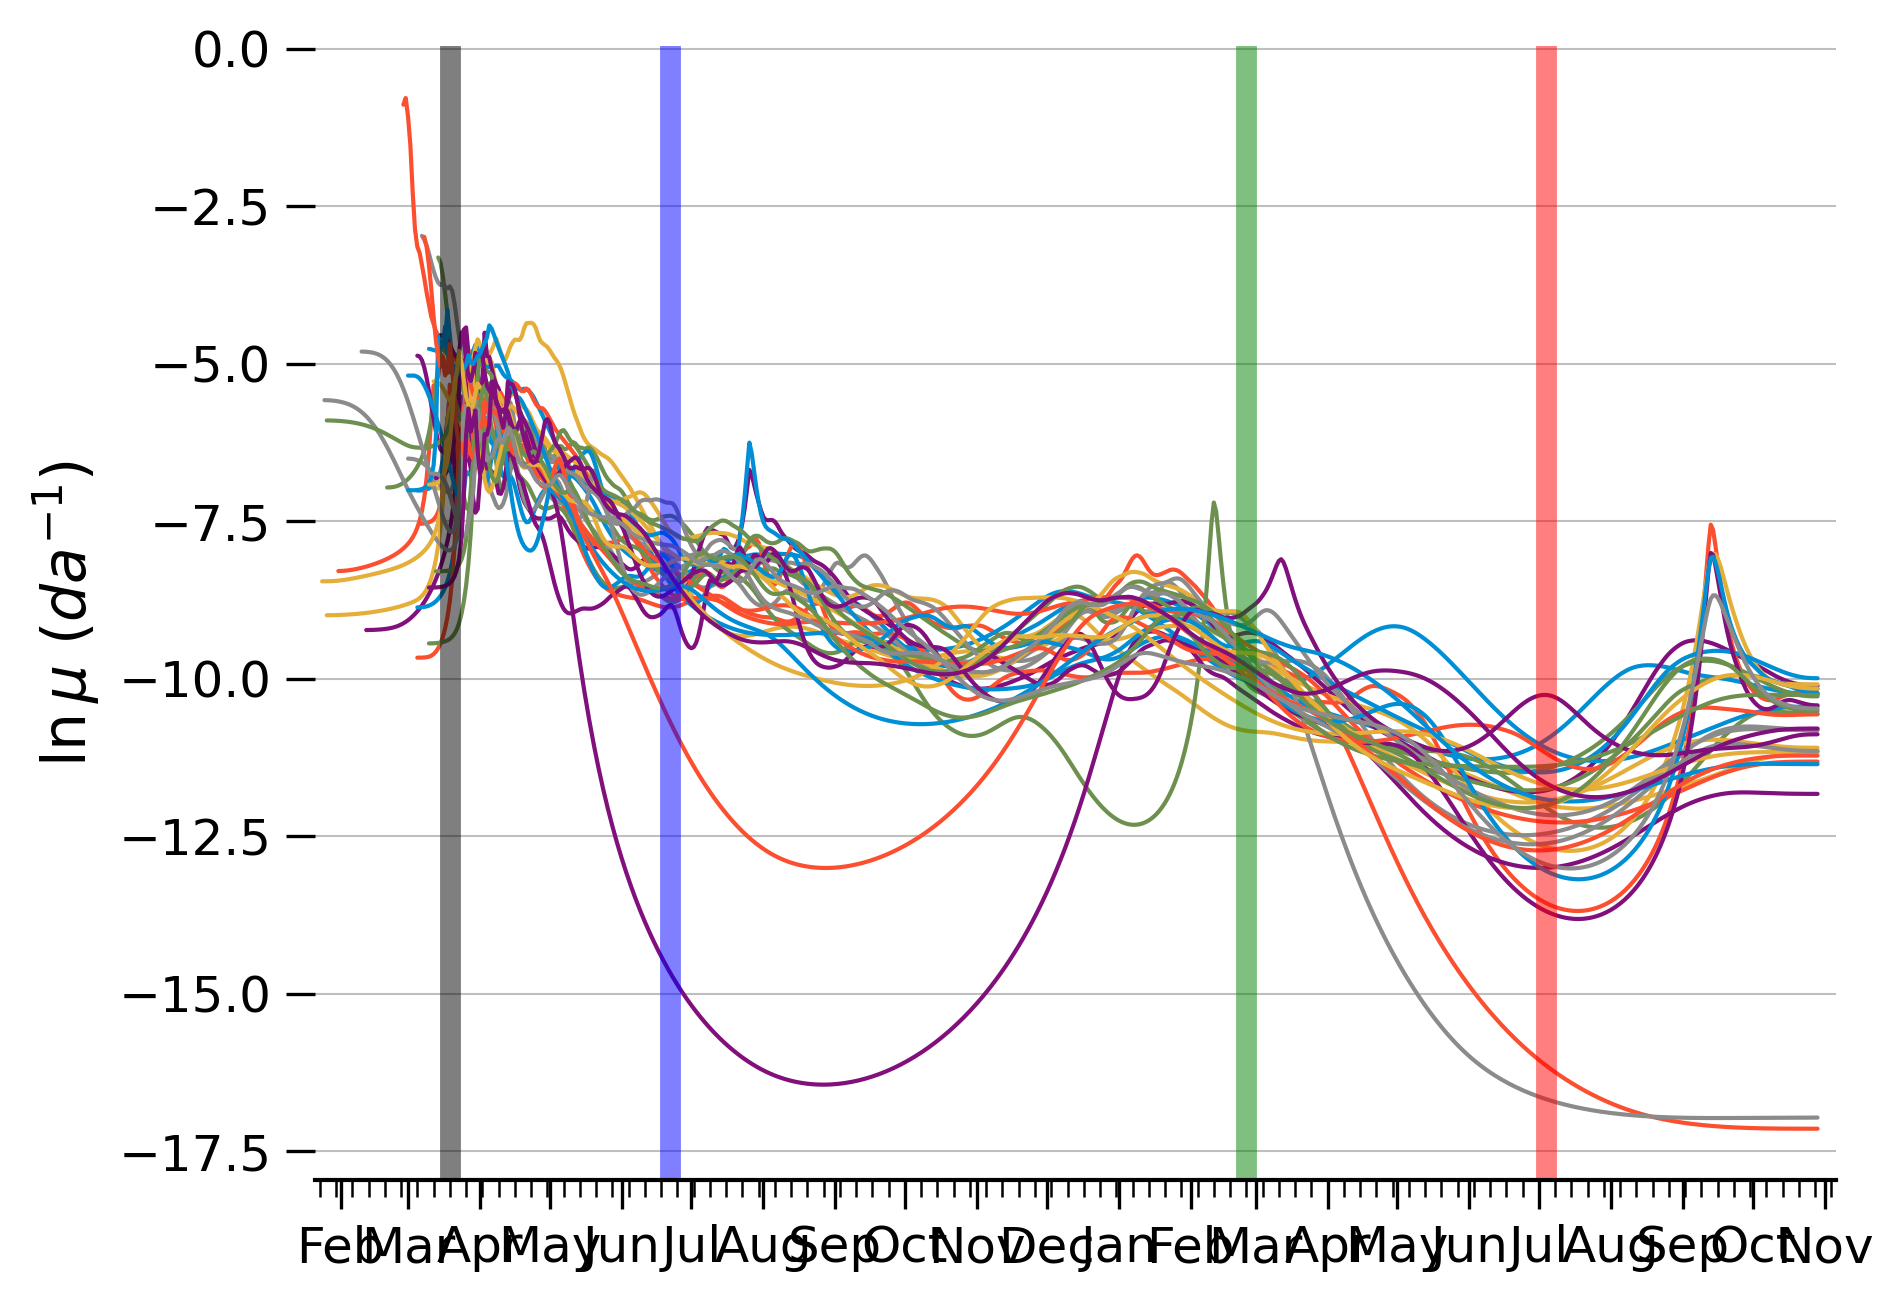
\includegraphics[height=0.40\textheight]{../Graphics/constrainID/logmu_summary_g.pdf}\\
%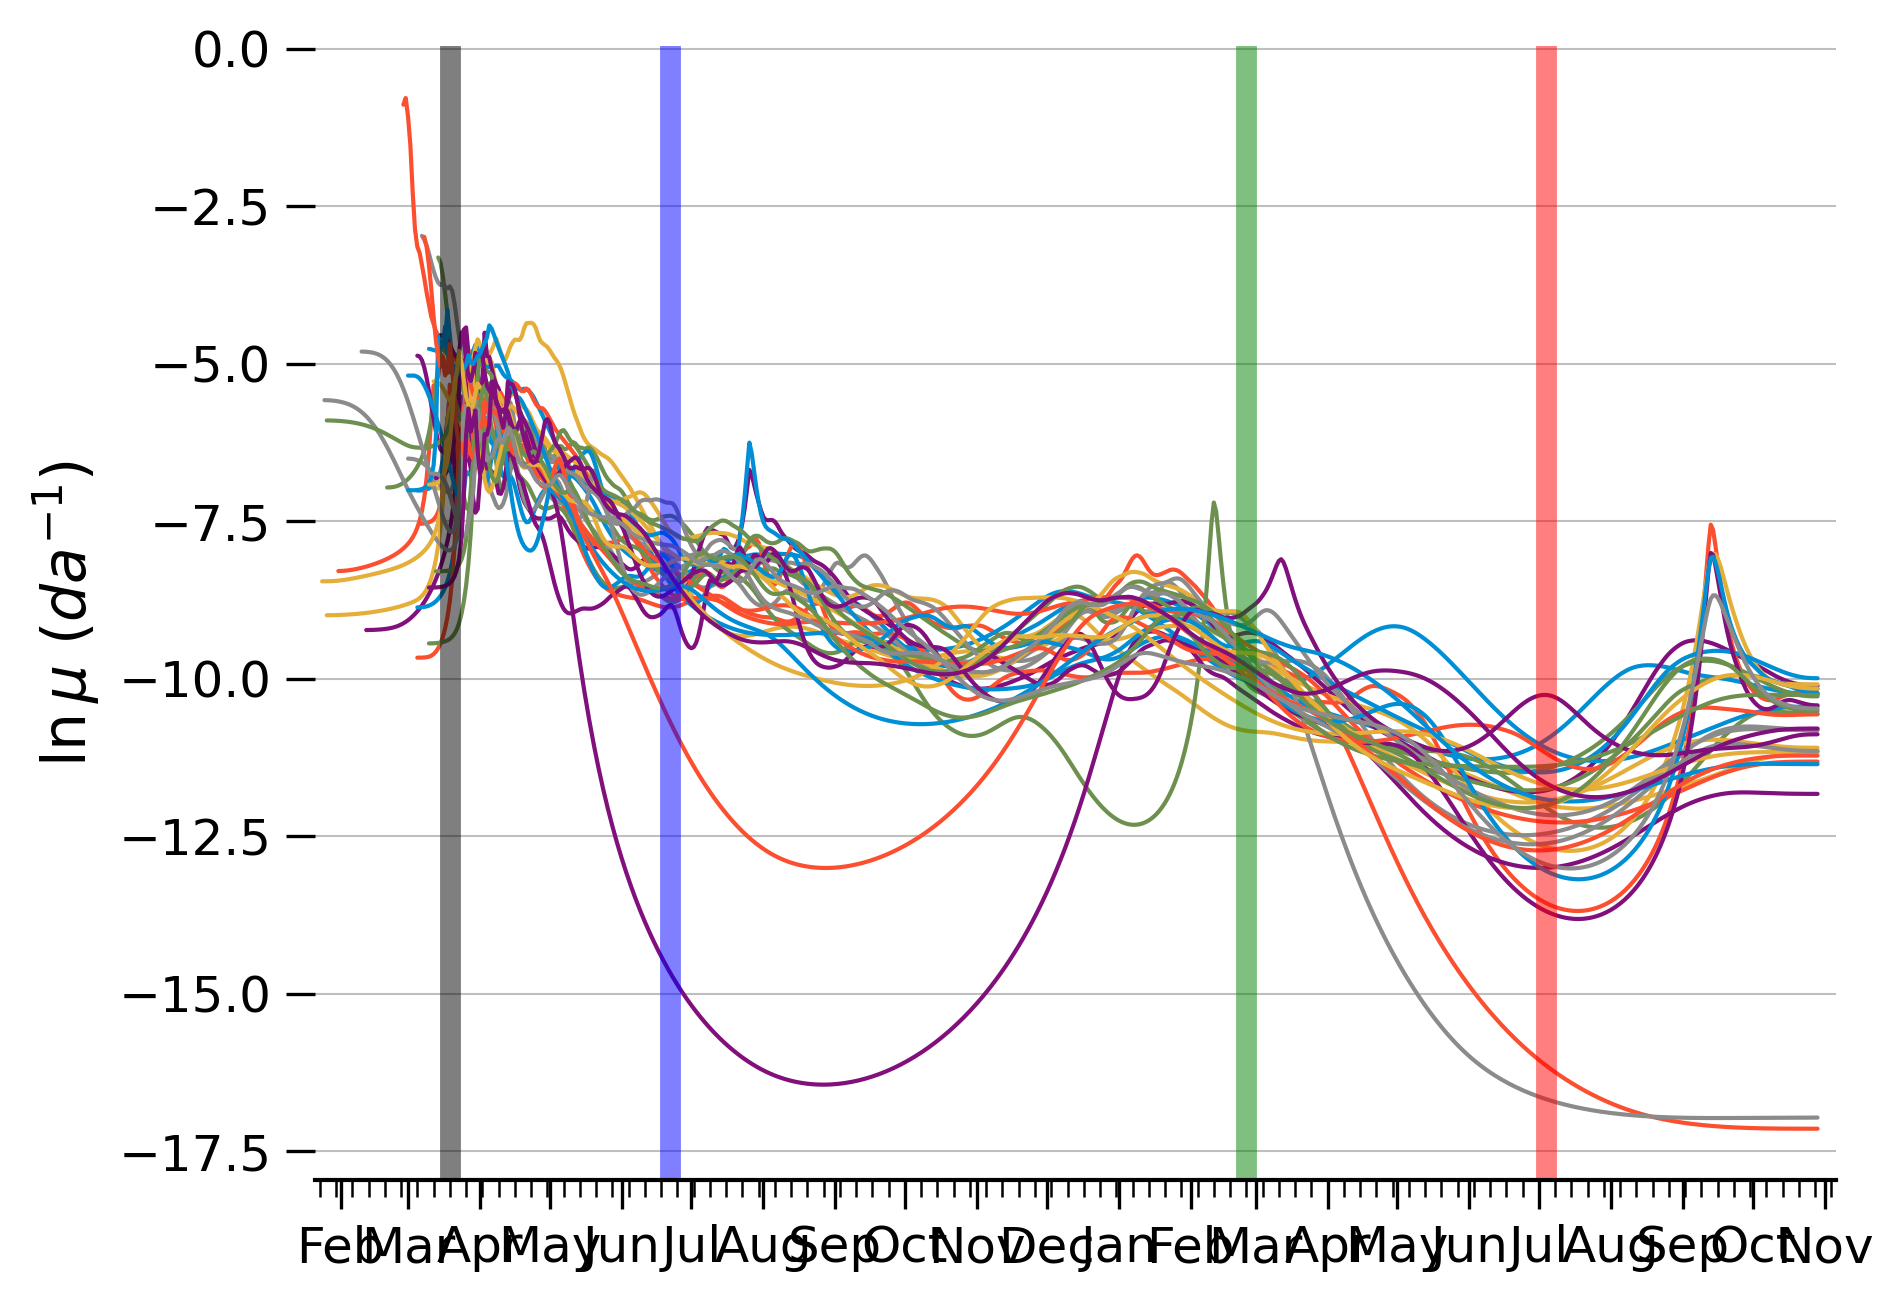
\includegraphics[width=1.00\textwidth]{../Graphics/constrainID/logmu_summary_g.pdf}\\
\end{center}
\caption{\label{fig:drates}
Estimated natural logarithms of the mortality rate for thirty two US
counties using the constrained \SSm\ model.
See Table~\ref{tab:namekey} for key to county abbreviations.
}
\end{figure}

\section*{Discussion}

Nonlinear statistical models with multiple parameters rely
on numerical methods to estimate parameters by searching for minima
%(hopefully finding only one) 
in the negative of the likelihood
function. The parameter values at the minima are considered to be
maximum likelihood estimators.  The minimization algorithms applied to
unconstrained \SSm\ do not reliably converge to solutions. The
standard deviations in the observation model are components of the
likelihood, and the algorithm pushes these parameters toward
unrealistically low estimates.  Setting the values of
\slI\ and \slD\ to arbitrarily small constants allows the
algorithm to estimate the other parameters.

The trends in estimated transmission rate Figure~\ref{fig:xrates} seem
reasonable. The extremely high transmission rates in March agree well
with doubling times reported in newspaper articles at the time.
The steady decline of transmission rates after shelter-in-place advice is 
also consistent with casual observation.
The transmission rates estimated for several counties appear to trend
upward, at least briefly, in July (figure~\ref{fig:xrates}). Counties
that display this upward deflection are also counties that have not
been successful in controlling spread of the outbreak

The incubation time of the Covid-19 virus is generally considered to be
about 14 days (\cite{Someone2020}).
The trends in Figure~\ref{fig:xrates} in conjunction with the
observed trends suggest that sustainable containment of
the pandemic does not occur unless the instantaneous transmission rate
is forced below \help{ $0.018 da^{-1}$}, that is, unless the doubling
time is greater than 35 days, approximately twice the incubation
period.

The magnitude and variability of the mortality rate estimates
(Figure~\ref{fig:drates})
at the start of the time series may be a result of variable lags
between between the first recorded case and the first recorded death.
The first recorded death in King Co. WA occurred on the second day of
the time series when four cases were recorded.
In contract, the first recorded death in Middlesex Co. MA occurred on
the sixteenth day of the time series when 177 cases were recorded.

%\clearpage


\clearpage
\printbibliography[title=References]
\clearpage

\appendixpage
\begin{appendices}


\section{Abbreviation Key}

\begin{table}[h!]
\caption{\label{tab:namekey}
Key to county name abbreviations.
}
\centering
\begin{tabular}{lll||lll}
\hline
Key&County&State&Key&County&State\\
\hline
AlCA&Alameda&CA&MuOR&Multnomah&OR\\
BeTX&Bexar&TX&NYNY&New York City&NY\\
BrFL&Broward&FL&NaNY&Nassau&NY\\
ClNV&Clark&NV&OaMI&Oakland&MI\\
CoIL&Cook&IL&OrCA&Orange&CA\\
DaTX&Dallas&TX&OrFL&Orange&FL\\
FrOH&Franklin&OH&PBFL&Palm Beach&FL\\
HaTX&Harris&TX&PhPA&Philadelphia&PA\\
HeMN&Hennepin&MN&RiCA&Riverside&CA\\
HiFL&Hillsborough&FL&SBCA&San Bernardino&CA\\
HoHI&Honolulu&HI&SCCA&Santa Clara&CA\\
KiWA&King&WA&SDCA&San Diego&CA\\
LACA&Los Angeles&CA&SaCA&Sacramento&CA\\
MDFL&Miami-Dade&FL&TaTX&Tarrant&TX\\
MaAZ&Maricopa&AZ&TrTX&Travis&TX\\
MiMA&Middlesex&MA&WaMI&Wayne&MI\\
\hline
\end{tabular}

\end{table}
\clearpage

\section{Estimation results}

\begin{sidewaystable}
\caption{\label{tab:cons}
Model results. Estimating $\beta$ and $\mu$ trends as random effects with 
constraints on  $\sigma_I$ and $\sigma_D$. 
Counties sorted in order of decreasing transmission rate ($\beta$).
Data updated 2020-08-04 from https://github.com/nytimes/covid-19-data.git.2020-08-04
}
\centering
{\scriptsize
%%%%%%%%%%%%%% :r ../fits/fit_table.tex


\begin{tabular}{lrrrrrrrrrrrr}
\hline
 County             &   $n$ &   $p_0$ &    $f$ &   $C$ &   $\sigma_\eta$ &   $\sigma_\beta$ &   $\sigma_\mu$ &   $\sigma_I$ &   $\sigma_D$ &   $\tilde\gamma$ &   $\tilde{\beta}$ &   $\tilde{\mu}$ \\
\hline
 Nassau, NY         & 151   & 0.0789  & -348   &     0 &          0.14   &            0.256 &         0.346  &        0.223 &       0.0953 &        -1.22e-08 &           0.00322 &        0.000241 \\
 New York City, NY  & 155   & 0.0833  & -310   &     0 &          0.161  &            0.217 &         0.36   &        0.223 &       0.0953 &        -2.36e-08 &           0.00533 &        0.000405 \\
 Wayne, MI          & 146   & 0.0544  & -336   &     0 &          0.14   &            0.229 &         0.16   &        0.223 &       0.0953 &        -1.8e-08  &           0.00619 &        0.000875 \\
 Oakland, MI        & 146   & 0.068   & -332   &     0 &          0.137  &            0.226 &         0.426  &        0.223 &       0.0953 &        -1.62e-08 &           0.0101  &        0.000594 \\
 Philadelphia, PA   & 146   & 0.102   & -340   &     0 &          0.126  &            0.175 &         0.425  &        0.223 &       0.0953 &        -2.42e-08 &           0.0106  &        0.000532 \\
 Middlesex, MA      & 151   & 0.105   & -357   &     0 &          0.124  &            0.237 &         0.371  &        0.223 &       0.0953 &        -1.25e-08 &           0.0107  &        0.000451 \\
 King, WA           & 157   & 0.00633 & -431   &     0 &          0.126  &            0.234 &         0.339  &        0.223 &       0.0953 &        -8.63e-09 &           0.013   &        0.000481 \\
 Franklin, OH       & 142   & 0.0629  & -419   &     0 &          0.102  &            0.157 &         0.3    &        0.223 &       0.0953 &        -1.76e-08 &           0.0208  &        0.00101  \\
 Honolulu, HI       & 150   & 0.166   & -484   &     0 &          0.0721 &            0.227 &         0.49   &        0.223 &       0.0953 &        -5.15e-08 &           0.0215  &        0.000174 \\
 Cook, IL           & 192   & 0.275   & -473   &     0 &          0.101  &            0.234 &         0.217  &        0.223 &       0.0953 &        -2.2e-07  &           0.0226  &        0.000466 \\
 Alameda, CA        & 155   & 0.141   & -465   &     0 &          0.0808 &            0.133 &         0.248  &        0.223 &       0.0953 &        -3.45e-08 &           0.0231  &        0.000527 \\
 Multnomah, OR      & 146   & 0.0272  & -497   &     0 &          0.0798 &            0.181 &         0.318  &        0.223 &       0.0953 &        -5.07e-08 &           0.0233  &        0.000362 \\
 Santa Clara, CA    & 185   & 0.204   & -586   &     0 &          0.071  &            0.237 &         0.274  &        0.223 &       0.0953 &        -1.55e-07 &           0.0246  &        0.000352 \\
 Los Angeles, CA    & 190   & 0.236   & -454   &     0 &          0.102  &            0.305 &         0.244  &        0.223 &       0.0953 &        -3.45e-07 &           0.0249  &        0.000423 \\
 San Diego, CA      & 175   & 0.244   & -430   &     0 &          0.0956 &            0.277 &         0.317  &        0.223 &       0.0953 &        -2.63e-07 &           0.0267  &        0.000719 \\
 Riverside, CA      & 149   & 0.06    & -482   &     0 &          0.09   &            0.138 &         0.183  &        0.223 &       0.0953 &        -2.72e-08 &           0.0294  &        0.000895 \\
 Palm Beach, FL     & 144   & 0.069   & -378   &     0 &          0.111  &            0.166 &         0.157  &        0.223 &       0.0953 &        -1.54e-08 &           0.0302  &        0.000942 \\
 Harris, TX         & 151   & 0.0921  & -373   &     0 &          0.102  &            0.197 &         0.322  &        0.223 &       0.0953 &        -2.44e-08 &           0.0302  &        0.000301 \\
 Miami-Dade, FL     & 145   & 0.11    & -342   &     0 &          0.133  &            0.197 &         0.206  &        0.223 &       0.0953 &        -1.08e-08 &           0.0308  &        0.000473 \\
 Orange, FL         & 143   & 0.0208  & -418   &     0 &          0.101  &            0.21  &         0.435  &        0.223 &       0.0953 &        -1.98e-08 &           0.0314  &        0.00024  \\
 Clark, NV          & 151   & 0.0724  & -436   &     0 &          0.1    &            0.158 &         0.218  &        0.223 &       0.0953 &        -3.3e-08  &           0.0319  &        0.000743 \\
 Travis, TX         & 143   & 0.0972  & -359   &     0 &          0.1    &            0.19  &         0.271  &        0.223 &       0.0953 &        -1.73e-08 &           0.0327  &        0.000319 \\
 Tarrant, TX        & 146   & 0.068   & -414   &     0 &          0.1    &            0.138 &         0.42   &        0.223 &       0.0953 &        -3.12e-08 &           0.0328  &        0.000335 \\
 Broward, FL        & 150   & 0.0728  & -391   &     0 &          0.107  &            0.167 &         0.447  &        0.223 &       0.0953 &        -2.15e-08 &           0.0333  &        0.000411 \\
 Orange, CA         & 191   & 0.313   & -519   &     0 &          0.0769 &            0.234 &         0.266  &        0.223 &       0.0953 &        -3.73e-07 &           0.0334  &        0.000732 \\
 Dallas, TX         & 146   & 0.0612  & -388   &     0 &          0.11   &            0.17  &         0.309  &        0.223 &       0.0953 &        -1.43e-08 &           0.0336  &        0.000504 \\
 San Bernardino, CA & 141   & 0.0634  & -406   &     0 &          0.0999 &            0.14  &         0.198  &        0.223 &       0.0953 &        -2.06e-08 &           0.0343  &        0.000794 \\
 Sacramento, CA     & 164   & 0.109   & -574   &     0 &          0.0666 &            0.174 &         0.252  &        0.223 &       0.0953 &        -8.02e-08 &           0.0343  &        0.000428 \\
 Hennepin, MN       & 144   & 0.103   & -359   &     0 &          0.114  &            0.207 &         0.402  &        0.223 &       0.0953 &        -1.24e-08 &           0.036   &        0.000917 \\
 Hillsborough, FL   & 155   & 0.16    & -461   &     0 &          0.0813 &            0.189 &         0.227  &        0.223 &       0.0953 &        -7.15e-08 &           0.0373  &        0.00065  \\
 Maricopa, AZ       & 190   & 0.283   & -482   &     0 &          0.0897 &            0.235 &         0.158  &        0.223 &       0.0953 &        -4e-07    &           0.0422  &        0.00188  \\
 Bexar, TX          & 173   & 0.224   & -478   &     0 &          0.0745 &            0.213 &         0.376  &        0.223 &       0.0953 &        -7.61e-08 &           0.0461  &        0.000393 \\
\hline
 Median             & 150.5 & 0.09465 & -418.5 &     0 &          0.101  &            0.202 &         0.3045 &        0.223 &       0.0953 &        -2.43e-08 &           0.0298  &        0.000477 \\
\hline
\end{tabular}


%%%%%%%%%%%%%%%%
}\end{sidewaystable}
\clearpage


\begin{sidewaystable}
\caption{\label{tab:uncons}
Model results. Estimating $\beta$ and $\mu$ trends as random effects
without constraints on  $\sigma_I$ and $\sigma_D$. 
Counties sorted in order of decreasing transmission rate ($\beta$).
Data updated 2020-08-04 from https://github.com/nytimes/covid-19-data.git.2020-08-04
}
\centering
{\scriptsize
%%%%%%%%%%%%%% :r ../fits/fit_table.tex

\begin{tabular}{lrrrrrrrrrrrr}
\hline
 County             &   $n$ &   $p_0$ &   $f$ &   $C$ &   $\sigma_\eta$ &   $\sigma_\beta$ &   $\sigma_\mu$ &   $\sigma_I$ &   $\sigma_D$ &   $\tilde\gamma$ &   $\tilde{\beta}$ &   $\tilde{\mu}$ \\
\hline
 Nassau, NY         & 151   & 0.0789  & -1190 &     1 &           0.231 &            0.603 &         10.3   &    0.000183  &     3.29e-08 &        -9.46e-09 &           0.00295 &       9.88e-05  \\
 New York City, NY  & 155   & 0.0833  & -1000 &     0 &           0.187 &            1.04  &          1.01  &    0.000436  &     0.000367 &        -2.73e-08 &           0.00476 &       0.000234  \\
 Oakland, MI        & 146   & 0.068   &  -836 &     1 &           0.16  &            1.55  &          1.18  &    9.12e-07  &     0.00426  &        -1.91e-08 &           0.00669 &       0.000318  \\
 Cook, IL           & 192   & 0.275   & -1100 &     1 &           0.116 &            3.68  &          0.992 &    8.16e-08  &     8.01e-05 &        -2.24e-07 &           0.00679 &       0.000201  \\
 Wayne, MI          & 146   & 0.0544  &  -856 &     1 &           0.192 &            1.15  &          1.46  &    0.000795  &     0.000936 &        -2.57e-08 &           0.00701 &       0.000362  \\
 Philadelphia, PA   & 146   & 0.102   &  -728 &     1 &           0.159 &            1     &          1.98  &    0.00274   &     0.00396  &        -3.1e-08  &           0.00964 &       0.000227  \\
 Middlesex, MA      & 151   & 0.105   &  -836 &     0 &           0.162 &            1.05  &          1.24  &    0.000663  &     0.00204  &        -1.56e-08 &           0.00995 &       0.000331  \\
 King, WA           & 157   & 0.00633 & -1080 &     1 &           0.147 &            0.474 &          0.909 &    0.00206   &     0.00224  &        -5.99e-09 &           0.0133  &       0.000455  \\
 Honolulu, HI       & 150   & 0.166   & -1480 &    10 &           0.116 &            4.87  &        117     &    0.000734  &     3.7e-06  &        -5.53e-08 &           0.0156  &       1.46e-11  \\
 Santa Clara, CA    & 185   & 0.204   & -1280 &     1 &           0.104 &            4.78  &          7.43  &    9.33e-08  &     2.29e-06 &        -1.53e-07 &           0.0158  &       1.16e-07  \\
 Sacramento, CA     & 164   & 0.109   &  -803 &    10 &           0.123 &            3.17  &          2.46  &    1.44e-06  &     0.0049   &        -8.81e-08 &           0.0183  &       0.00016   \\
 Multnomah, OR      & 146   & 0.0272  &  -894 &     1 &           0.119 &            0.896 &          3.35  &    0.0036    &     0.00226  &        -6.79e-08 &           0.0234  &       5.44e-05  \\
 Franklin, OH       & 142   & 0.0629  &  -819 &     1 &           0.123 &            0.462 &          1.3   &    0.00255   &     0.00368  &        -1.42e-08 &           0.0239  &       0.000575  \\
 Los Angeles, CA    & 190   & 0.236   &  -971 &     1 &           0.242 &            0.889 &          0.983 &    2.22e-06  &     0.00661  &        -3.77e-07 &           0.024   &       0.000399  \\
 Alameda, CA        & 155   & 0.141   &  -905 &     1 &           0.131 &            3.61  &         20.3   &    2.65e-05  &     6.68e-08 &        -3.95e-08 &           0.0241  &       9.44e-10  \\
 San Diego, CA      & 175   & 0.244   &  -850 &     1 &           0.161 &            1.08  &          1.23  &    4.71e-06  &     0.0103   &        -2.91e-07 &           0.0247  &       0.000335  \\
 Bexar, TX          & 173   & 0.224   &  -689 &     1 &           0.131 &            2.61  &          1.44  &    0.000397  &     0.0103   &        -7.18e-08 &           0.0261  &       0.000256  \\
 Orange, CA         & 191   & 0.313   &  -878 &     1 &           0.127 &            1.54  &          0.961 &    6.16e-06  &     0.053    &        -4.02e-07 &           0.0268  &       0.000509  \\
 Orange, FL         & 143   & 0.0208  &  -710 &     1 &           0.119 &            0.678 &          1.08  &    0.0015    &     0.0373   &        -2.3e-08  &           0.027   &       0.000192  \\
 Clark, NV          & 151   & 0.0724  &  -662 &    10 &           0.148 &            1.5   &          5.31  &    0.00247   &     1.25e-05 &        -4.16e-08 &           0.0276  &       0.000322  \\
 Tarrant, TX        & 146   & 0.068   &  -662 &     1 &           0.14  &            1.24  &          1.34  &    0.00891   &     0.00326  &        -3.79e-08 &           0.0283  &       0.000269  \\
 Harris, TX         & 151   & 0.0921  &  -429 &     1 &           0.116 &            0.27  &          0.965 &    0.156     &     0.0215   &        -2.11e-08 &           0.0297  &       0.000289  \\
 Palm Beach, FL     & 144   & 0.069   &  -507 &     0 &           0.137 &            0.337 &          1.31  &    0.0822    &     0.00588  &        -1.16e-08 &           0.0302  &       0.000525  \\
 San Bernardino, CA & 141   & 0.0634  &  -567 &     1 &           0.146 &            1.74  &          2.74  &    0.0051    &     0.00586  &        -1.74e-08 &           0.0304  &       0.000207  \\
 Miami-Dade, FL     & 145   & 0.11    &  -722 &    10 &           0.156 &            0.639 &          0.961 &    6.89e-06  &     0.00814  &        -9.55e-09 &           0.0313  &       0.000447  \\
 Hennepin, MN       & 144   & 0.103   &  -726 &     0 &           0.14  &            0.72  &          1.35  &    0.00522   &     0.00203  &        -9.13e-09 &           0.0314  &       0.00048   \\
 Riverside, CA      & 149   & 0.06    &  -683 &     1 &           0.113 &            1.25  &          5.23  &    0.0174    &     2.17e-05 &        -2.61e-08 &           0.0317  &       0.000718  \\
 Maricopa, AZ       & 190   & 0.283   &  -932 &     1 &           0.105 &            1.23  &          1.26  &    5.43e-06  &     0.0164   &        -4.2e-07  &           0.0322  &       0.000596  \\
 Travis, TX         & 143   & 0.0972  &  -394 &     1 &           0.14  &            0.107 &          1.44  &    0.177     &     0.0131   &        -1.67e-08 &           0.0329  &       0.000265  \\
 Hillsborough, FL   & 155   & 0.16    &  -653 &     0 &           0.111 &            1.11  &          1.28  &    0.00477   &     0.0169   &        -7.24e-08 &           0.0329  &       0.000393  \\
 Broward, FL        & 150   & 0.0728  &  -584 &     1 &           0.13  &            0.23  &          1.63  &    0.0759    &     0.00289  &        -2.03e-08 &           0.0331  &       0.000275  \\
 Dallas, TX         & 146   & 0.0612  &  -529 &     1 &           0.13  &            0.303 &          1.26  &    0.0757    &     0.00757  &        -1.04e-08 &           0.0349  &       0.000342  \\
\hline
 Median             & 150.5 & 0.09465 &  -811 &     1 &           0.134 &            1.065 &          1.325 &    0.0011475 &     0.00382  &        -2.67e-08 &           0.0254  &       0.0003035 \\
\hline
\end{tabular}

%%%%%%%%%%%%%%%%
}\end{sidewaystable}



\clearpage
\section{Diagnostic Plots}

\begin{figure}[h!]
\begin{center}
\includegraphics[width=1.00\textwidth]{../Graphics/constrainID/NassauNY_TMB_estimates_a.pdf}
\end{center}
\caption{\label{fig:estsNaNYca}
Diagnostic plots of model estimates for Nasssau County, NY, 
with constraints of the observation model variance, 
\slI~$ = 0.223$ and \slD~$= 0.00953$. 
Cases and deaths plotted on arithmetic scale.
See page~\pageref{pp:diagexpl} for explanation of figure.
}
\end{figure}
\clearpage

\begin{figure}
\begin{center}
\includegraphics[width=1.00\textwidth]{../Graphics/constrainID/Miami-DadeFL_TMB_estimates_a.pdf}
\end{center}
\caption{\label{fig:estsMDFLca}
Diagnostic plots of model estimates for Miami-Dade County, FL
with constraints of the observation model variance, 
\slI~$ = 0.223$ and \slD~$= 0.00953$. 
Cases and deaths plotted on arithmetic scale.
See page~\pageref{pp:diagexpl} for explanation of figure.
}
\end{figure}

\begin{figure}[h!]
\begin{center}
\includegraphics[width=1.00\textwidth]{../Graphics/unconstrained/NassauNY_TMB_estimates.png}
\end{center}
\caption{\label{fig:estsNaNYu}
Diagnostic plots of model estimates for Nasssau County, NY, 
without constraints of the observation model variance. 
See page~\pageref{pp:diagexpl} for explanation of figure.
}
\end{figure}
\clearpage

\begin{figure}
\begin{center}
\includegraphics[width=1.00\textwidth]{../Graphics/unconstrained/Miami-DadeFL_TMB_estimates.png}
\end{center}
\caption{\label{fig:estsMDFLu}
Diagnostic plots of model estimates for Miami-Dade County,FL,
without constraints of the observation model variance. 
See page~\pageref{pp:diagexpl} for explanation of figure.
}
\end{figure}

\end{appendices}

\end{document}


%An integer code. 0 indicates successful completion (which is always the case for "SANN" and "Brent"). Possible error codes are
%
%1
%
    %indicates that the iteration limit maxit had been reached.
%10
%
    %indicates degeneracy of the 
%

Whether the available data are sufficiently informative to enable
estimation of the model parameters is a critical aspect of the
evaluation of any statistical model.
The speed at which the Covid-19 pandemic spread during the first
quarter of
2020 means that the length of the time series doubled during
the development of this model. The capability of the
model improve conveniently during the model development period,
but whether the improvement is
attributable to changes in model structure or to the increase in the
length of the time series is unclear. This ambiguity influenced the
development of the model.
